\documentclass[12pt, a4paper]{article} 

\usepackage[utf8]{inputenc}


\usepackage{geometry} % to change the page dimensions
\geometry{a4paper} % or letterpaper (US) or a5paper or....

\usepackage{graphicx} % support the \includegraphics command and options

\usepackage{booktabs} % for much better looking tables
\usepackage{array} % for better arrays (eg matrices) in maths
\usepackage{paralist} % very flexible & customisable lists (eg. enumerate/itemize, etc.)
\usepackage{verbatim} % adds environment for commenting out blocks of text & for better verbatim
\usepackage{subfig} % make it possible to include more than one captioned figure/table in a single float
% These packages are all incorporated in the memoir class to one degree or another...
%\usepackage{caption}
%\usepackage[list=true,listformat=simple]{subcaption}
\usepackage{float}
\usepackage{listings}
\usepackage{natbib}

%citation style
\bibliographystyle{apalike}
\bibpunct{[}{]}{;}{a}{,}{,}

\usepackage{amsmath, amssymb}% for mathematical symbols
\usepackage[colorlinks=true,linkcolor=black,urlcolor=black, citecolor=black]{hyperref} % for hyperreferences with black color
%\usepackage[T1]{fontenc} % Uncomment for norwegian document
%\usepackage[norsk]{babel} %

%%% HEADERS & FOOTERS
\usepackage{fancyhdr} % This should be set AFTER setting up the page geometry
\pagestyle{fancy} % options: empty , plain , fancy
\renewcommand{\headrulewidth}{0pt} % customise the layout...
\lhead{}\chead{}\rhead{}
\lfoot{}\cfoot{\thepage}\rfoot{}

%%% SECTION TITLE APPEARANCE
\usepackage{sectsty}
\allsectionsfont{\sffamily\mdseries\upshape} % (See the fntguide.pdf for font help)
% (This matches ConTeXt defaults)

%%% ToC (table of contents) APPEARANCE
\usepackage[nottoc,notlof,notlot]{tocbibind} % Put the bibliography in the ToC
\usepackage[titles,subfigure]{tocloft} % Alter the style of the Table of Contents
\renewcommand{\cftsecfont}{\rmfamily\mdseries\upshape}
\renewcommand{\cftsecpagefont}{\rmfamily\mdseries\upshape} % No bold!



%%% END Article customizations

%%% The "real" document content comes below...

%\title{Specialization project report}
%\author{Hong-Dang Lam}
%\date{} % Activate to display a given date or no date (if empty),
         % otherwise the current date is printed 

\begin{document}
\begin{titlepage}


% Upper part of the page. The '~' is needed because \\
% only works if a paragraph has started.

\textsc{\LARGE Norwegian University of Science and Technology}\\[1.5cm]

\textsc{\Large TDT4501 Specialization Project}\\[0.5cm]

% Title

{ \huge \bfseries Specialization project report \\[0.4cm] }


% Author and supervisor
\noindent
\begin{minipage}{0.4\textwidth}
\begin{flushleft} \large
\emph{Author:}\\
Hong-Dang \textsc{Lam}
\end{flushleft}
\end{minipage}%
\begin{minipage}{0.4\textwidth}
\begin{flushright} \large
\emph{Supervisors:} \\
Keith \textsc{Downing}\\
Christian \textsc{Skjetne}
\end{flushright}
\end{minipage}\\

\vfill

% Bottom of the page
{Fall 2014\\\large \today}

\end{titlepage}




\pagenumbering{gobble}
\pagenumbering{Roman}
\newpage
\begin{abstract}
INTELLIGENT ROBOTICS: Swarm Intelligence
Students will work with groups of simple agents (e.g. simulated or physical robots) to investigate the emergence of global structure from local interactions. No global controller will dictate the agents' actions.


\end{abstract}

\newpage
\tableofcontents
\newpage
\listoffigures
\newpage
\listoftables
\newpage
\pagenumbering{arabic}
%1 introduction
\section{introduction}
insert introduction here

%2 related works
\section{Background}
Background introduction

\subsection{Swarming}
Swarm, swarming, swarm intelligence, swarm optimization or swarm robotics are terms used for simple (preferably cheap) robots which can only do simple tasks. However the power of these robots lies in the numbers. The robots might not be able to do an advanced task alone, but together they might be able complete advanced tasks. For instance, one robot might not be able to push a heavy box by itself, but with the help of other robots they might be able to push the box.
Each robot are allowed to communicate with each other, but they do not need to communicate. There are no centralized controller that controls the robot, each one needs to find out what it needs to do by itself or by communicating with the other robots. The idea behind these simple cheap robots are that they can easily be mass produced, interchangeable, modularized and disposable. If one robot is malfunctioning or broken, it would not affect the rest of the swarm. It is therefore no single point of failure in a swarm, and the system is very scalable because robots can easily be added to the system.
Swarm robotics are often very computer efficient, because they each have their own processor. This reduces the computational overhead. 

\subsection{Boids}
In 1986, Craig W. Reynolds created something called Boids, which stands for \textbf{B}ird-\textbf{oid} object\textbf{s}. Boids are particles that would behave like birds, they would try to flock and fly together without colliding. This was done by using 3 simple behaviors;
\begin{description}
    \item[Separation]
        Each individual will steer away from the other individual if they were too close to each other. This ensure that they do not collide with their neighbors.
    \item[Alignment]
        In a neighborhood (for instance a radius around the individual or the $X$ nearest individuals) find the average angle of the neighborhood and align itself so its angle matches the average angle of the neighborhood.
    \item[Cohesion]
        Steer towards the average position of the other individuals in your neighborhood. This makes the Boids stay in the flock.
\end{description}
\begin{figure}[H]
    \centering
    \subfloat[Separation ]{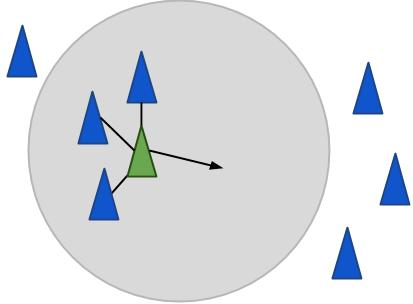
\includegraphics[width=0.3\textwidth]{images/boid_separation.jpg}}
    \hfill
    \subfloat[Alignment ]{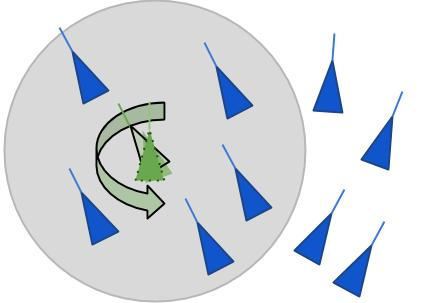
\includegraphics[width=0.3\textwidth]{images/boid_alignment1.jpg}}
    \hfill
    \subfloat[Cohesion ]{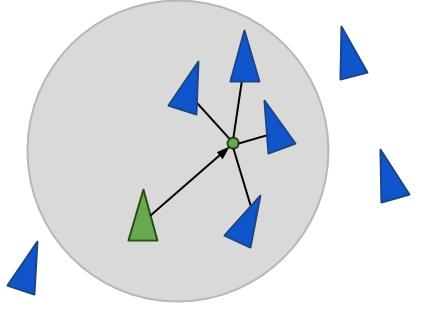
\includegraphics[width=0.3\textwidth]{images/boid_cohesion.jpg}}
            \caption[Boids behavior]{The three behaviors of the Boids}
            \label{fig:boidbehavior}
\end{figure}

The three behavior is per individual Boid, which means that each particle/Boid has to calculate where they are going to fly by checking all the other Boids position and rotation and then act accordingly. Which makes this algorithm $ O(n^2)$ for every frame. 
Reynolds have tried to make the algorithm less computational intensive by putting the Boids into grids with Spatial Hashing. An example of could be to put all the Boids that has a position $0<x<1$ and $0<y<1$ on the lower left grid, and the ones that has a $1<x<2$ in the next position etc. Using this grid, each Boids in a cell only needs to take the adjacent grids into consideration when checking their neighborhood. 
\begin{figure}[h!]
    \centering
    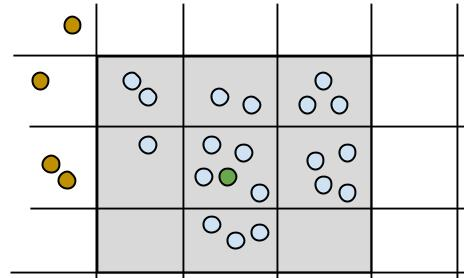
\includegraphics[width=0.8\linewidth]{images/boid_spatialhash}
    \caption{Boids in grids using spatial hash} \label{fig:spatialhash}
\end{figure}
As illustrated in the figure, the green Boid only needs to check the gray Boids that surrounds its own cell, it does not need to check the rotation and position of the orange/brown Boids outside of the gray box, because they are too far away to be considered a part of its neighborhood.

In another paper a different technique were used to optimize 3D swarms, a method using neighborhood grids.\\

Other optimization has been made as well, like the neighborhood grid.
Each Boids to cell ratio would be 1 to 1, that is for every cell, there would be at max 1 Boid. Each Boid would have their respective cell based on their position in space, for instance a Boid with low $x$-value would be on the left of a Boid with higher $x$-value, and Boids who are closer to each other in geometric space would be stored closer to each other in the grid. To obtain this, the Boids needed to be sorted. Odd Even sort and Bitonic sort were used as the sorting algorithm.\\
Of the two sorting algorithm, Odd Even sort was faster, but not very precise. More than 10\% of the entities were placed in the wrong cell. The paper did an odd even sort algorithm for each axis, that is one odd even sort for x, y and z in paralell.\\
Bitonic Sort on the other hand was slower, but a lot more precise. Less than 1\% of the entities were placed in wrong cell. The reason for placing a Boid in the wrong cell is due to way the sorting works, it sorts all the entities in one axis first, then a second axis and then the third last axis. For instance sorting on $x$-values first, for the $y$-values, then the $z$-values. When swapping one of the latter axises it might mess up the sorting of one of the other axises.

After the Boids were placed in their corresponding grid, the work could be distributed to the GPU which would calculate where each Boids' new location and rotation would be based on their adjacent neighbor depending on the Moore radius.
The paper tried to vary the number of Boids from 1,000 to 1,000,000 and they had 4 types of Boids. The same types of Boids would try to flock with each other while different types of Boids would try to avoid each other.
They were able to see a speedup compared to the spatial hashing method used by Reynolds, but the Boids were not rendered as a bird or an object, only as a primitive shape. They didn't mention if they tried to add non moving obstacles in their test. Due to the high percentage of Boids being placed in the wrong cell when using odd even sort, a lot of Boids would crash into their neighbor during the test run. However using the neighborhood grid method on GPU, real time simulation of 1 million Boids were possible (6-8 fps).\\

In the paper "steering behaviors for autonomous character" Reynold discusses that an autonomous character, which is a type of autonomous agent are agents that have some ability to improvise their actions. That means that these agents do not have their actions scripted in advance.
These autonomous agents can have various 
in another paper he discussed various behaviours for autonomous steering, like seek, chase, flee etc.




In the paper named "not bumping into things" W. Reynolds discusses how to perform obstacle avoidance, that is obstacles that are placed in the environment which is not a boid. These obstacles are usually static, that is non moving obstacles. He starts out with the idea of a forcefield around the obstacle which he calls the \textit{steer away from surface} approach. The idea is to have every obstacle emit a forcefield around itself which pushed the boids away. For instance if a boid is flying toward an obstacle, the obstacle would push the boid to one side of itself. However this force field method would not work if the boid flew straight into an obstacle, because the forcefield force would be straight opposite of the direction the boid is flying thus making the boid deaccelerate until it stopped.
The next obstacle avoidance technique Reynold discussed is the curb feeler technique or steer along the wall technique. The idea is to have a feeler that would detect an obstacle before the boid would crash into it, then turn the boid away from the obstacle. This can be compared to walking down a dark alleyway where you'll reach your hand out to feel the walls around you and navigates through the alleywall just by feeling the wall(s).
The last technique for navigating and avoiding obstacles discussed in this paper was image processing. Images could processed in real time to a grayscale image where white would signify an obstacle. The algorithm would start with the center of the image, if this was a white pixel it would start to search outwards in a spiral to find either a gray pixel or a black one and then turn the boid in this direction. This could also be combined with a \textit{Z-buffer image} which gives us a map of the distances to obstacles that lies in front of the boid, this z-buffer iamge can be obtained by radar, sonar or similar technology. One interesting way of using the Z-buffer image is to implement a "steer towards the longest clear path". However using this technique without any form of planning or learning might lead the boid into a local cavity which might be a dead end.

In the paper Distributed physics-based control of swarms of vehicles by W. Spears and D. Spears a self emergent system is formed using simple attractive and repulsion force for each particle. The idea behind their system was to create an artificial physics framework (AP) that would simulate a physical system. In their paper they had the particles attract other particles that were farther away than distance \textit{r} and a repulsive force is applied if the particles are closer than distance \textit{r}. This leads to the particles always being at distance \textit{r} from each other which will form a hexagonal lattice. They also tried out making patterns, but had to introduce a concept of spin; each particle were either spin "down" or spin "up". Opposite spins would attract each other if the distance was greater than \textit{r} and repel each other if the distance is less than \textit{r}. If the particles had opposite spin the distance would be $\sqrt{2}r$. This means that all the vertical particles would be alternating between spin up and spin down, the same goes for the particles in the horizontal space. The diagonal particles on the other hand will have the same spins as their diagonal neighbors.

In the paper "V-like formation in flocks of artificial birds" by A. Nathan and V. Barbosa bird flocking is discussed. They ran a simulation that where each bird individual had 3 simple rules: 
\begin{itemize}
    \item Coalescing rule \\
        The birds should try to seek the proximity of the nearest bird.
    \item Gap-seeking rule \\
        If rule 1, the coalescing rule is not applicable anymore the bird should find a position with unobstructed view -  that is, the bird should be able to see in front of it without anything being in the way.
    \item Stationing rule \\
        Try to stay in place.
\end{itemize}
These rules would make sure that the birds were able to flock and form different shapes. The only thing that was common between the different runs in this paper was that the bird behind would be a little bit behind and slightly left or right of the bird in front (following rule \#2). A lot of different shapes was obtained during the runs, the birds flocked and formed a V-shape, a diagonal line, an inverted V-shape etc.

\subsection{Family bird: A heterogenous simulated flock}
This paper says that bird flocks and fish schools seems to be very complex, but the mechanics are very simple as illustrated by Reynold. Only a few simple rules will create flocks that flock together and splits up to avoid obstacles. These flocks are not spectacular or mind blowing compared to the flocks found in nature, due to the rigid motion of each individual. To tackle the artificialness of each individual, Heppner introduced randomness to the motion of the individuals, defending it by saying that these randomness simulates wind gust, random obstacles and other factors. 
However the authors of this paper does not agree with this approach because wind gusts will affect the whole flock, not just a random single individual at random. Even with these randomness added, the flock still does not seem lifelike enough compared to their counterpart found in nature. The reason for the lack of breathtaking in these flocking algorithms are that the individuals all have the same characteristics. In nature each individual will have different size, age, form and shape. 
Usually in flocking algorithms, each individual takes into account where all the other entities are and then act accordingly. In nature, each individual might have limited information about the flock, it might only be able to gain so much from its vision due to other flock members being occluded or not able to hear some of the other individuals due to noise or other factors.
This paper runs a simulation with different types of bird , where social relations are a factor and individuals might be solitary or social. Social individuals are entities who would like to stay close to members of its own social group, for instance a social dove will want to stay with other doves. Solitary individuals on the other hand does not care about staying with its own flock and might drift to another flock. For instance a solitary dove might fly amongst hawks or other types of birds. A flock in this paper are defined as a group where the individuals affect each other in the same group. The simulation they ran varied between all solitary birds to 4 types of different social birds.

\subsection{Particle Swarm Optimization}
Swarms has a lot of potential, not necessary only on robotics but swarms can be used to optimize problem, hence the name particle swarm optimization (PSO). PSOs are used to solve problems where optimization are needed. The idea behind PSOs are to have a swarm of particles spawn at random positions in the search space, and then let them fly around searching for solutions. Each particle will know the best solution it have found so far, and the best solution that is found globally. In some PSO implementations a local best found solution is also known amongst the individual. This local best solution is the best solution amongst a subgroup of individuals and can change for a particle depending on the position of the particle.

\subsection{Other swarming animals}
\subsubsection{fishes}
In this paper Xiaoyuan Tu explains how fishes form schools and how different intentions make the fish behave the way they do. He starts out with explaining how a fish and how the simulator is constructed, the math behind it and how the motor controllers work. For the simulation there's different types of fishes, some of them are predators and some of them are preys. The name explains itself, but to be clear, predators are larger fishes which tries to eat other smaller preys. Each fish has a 300 degrees, where it can see in front of it and has a blind spot directly behind it. 
The range of the vision is also limited and might be occluded by other objects. Each fish has a intention generator, which basically is a flowchart of what the fish needs to do. The prey and predator fish have different intention generators. The predators do not get preyed upon, and thus does not need to look out for other predators, therefore are the intentions of escaping, mating and schooling with other fishes of the same species are disabled. The reason for disabling mating is because there's no need for new predator fishes because they don't die in this simulation. They also don't need to school with other predators because they are not in danger, and don't need the extra survivability.\\
Whenever a predator sees a prey it will chase the prey if the cost of reaching it is minimal, if it's too much, it will not bother chasing. \\
Preys on the hand needs the extra survivability, and will try to school with the other fishes if it detects a predator nearby. Each fish will then try to stay a certain distance from each other, which is roughly on body length in distance. Then the fishes will try to adjust its speed and direction so it matches the other members. When this school of fish encounter an obstacle, they individual fishes will try to avoid this obstacle, this might lead to the school splitting up and rejoining after they have avoided the obstacle. \\
A third type of fish introduced here are the pacifists fish. This one differs from the other two type in that the intention of mating is activated while escaping and schooling are deactivated.
The paper describes that there are male and female fishes, and the two behavior which can occur when the fishes start to mate. A behavior named \textit{nuzzling} where the male fish seeks the female and nudges her abdomen until she's ready to spawn, and \textit{spawning ascent} where the female swims repeatedly to the surface while releases gametes. The paper also describes in detail how the fishes select potential partners and how they try to impress each other for mating purposes.

\subsubsection{Ant swarms/colonies}
Ant swarms behaves differently than other types of swarms, ants do not try to form formations for survival in the same way that birds and fishes do. Ant swarming are mostly about their foraging behavior, that is how they find food for their colony. Each ants' goal is the survival of the colony rather than the survival of each individual. When ants tries to find food, they scatter the area by walking in random manner. While exploring the ants leave behind a chemical on the ground, a so called pheromone that the other ants will be able to feel/smell. This pheromone will slowly but surely dissipate. Whenever the explorer ant find a food source, it will evaluate the quality of the food before returning to the anthill. During the return trip, pheromones are reapplied to the path, but the amount is adjusted based on the evaluation of the food, better food will yield higher pheromone. This method will ensure that the rest of the ants will take the shortest path from the anthill to the food.
%3 chirp robots
\section{ChIRP. Robot}
The ChIRP (CHeap and Interchangable Robotic platform) robot is a robot developed by the CRAB lab, which is part of the artificial intelligence group at the Department of Computer and Information Science (IDI) at the Norwegian University of Science And Technology (NTNU).

The purpose behind the development of the ChIRP robot is to research sub symbolic AI, whether it is swarming or evolution. Sub symbolic AI are algorithms and AI inspired by nature or biology. This covers Artificial Neural Network inspired from the human brain, swarm robots inspired from bird flocks, ant colonies, fish schools etc. Evolution and genetic programming are also one of topics included in sub symbolic AI.
The robots' data schema and source code are all open source and can be found at \href{http://chirp.idi.ntnu.no}{chirp.idi.ntnu.no}. The robot consist of a printed circuit board (PCB), 2 motors which controls the 2 wheels on each side of the robot.
Modules like LED lights and various sensors can be soldered on the PCB thus the robots' are easily modifiable, and the robots can have multiple layers with different sensors so it is not limited to have only light sensors or infrared sensors. The standard ChIRP robot comes with 8 infrared-LEDs and 8 infrared receivers as seen on figure \ref{fig:chirpAbove}.
\begin{figure}[H]
\centering
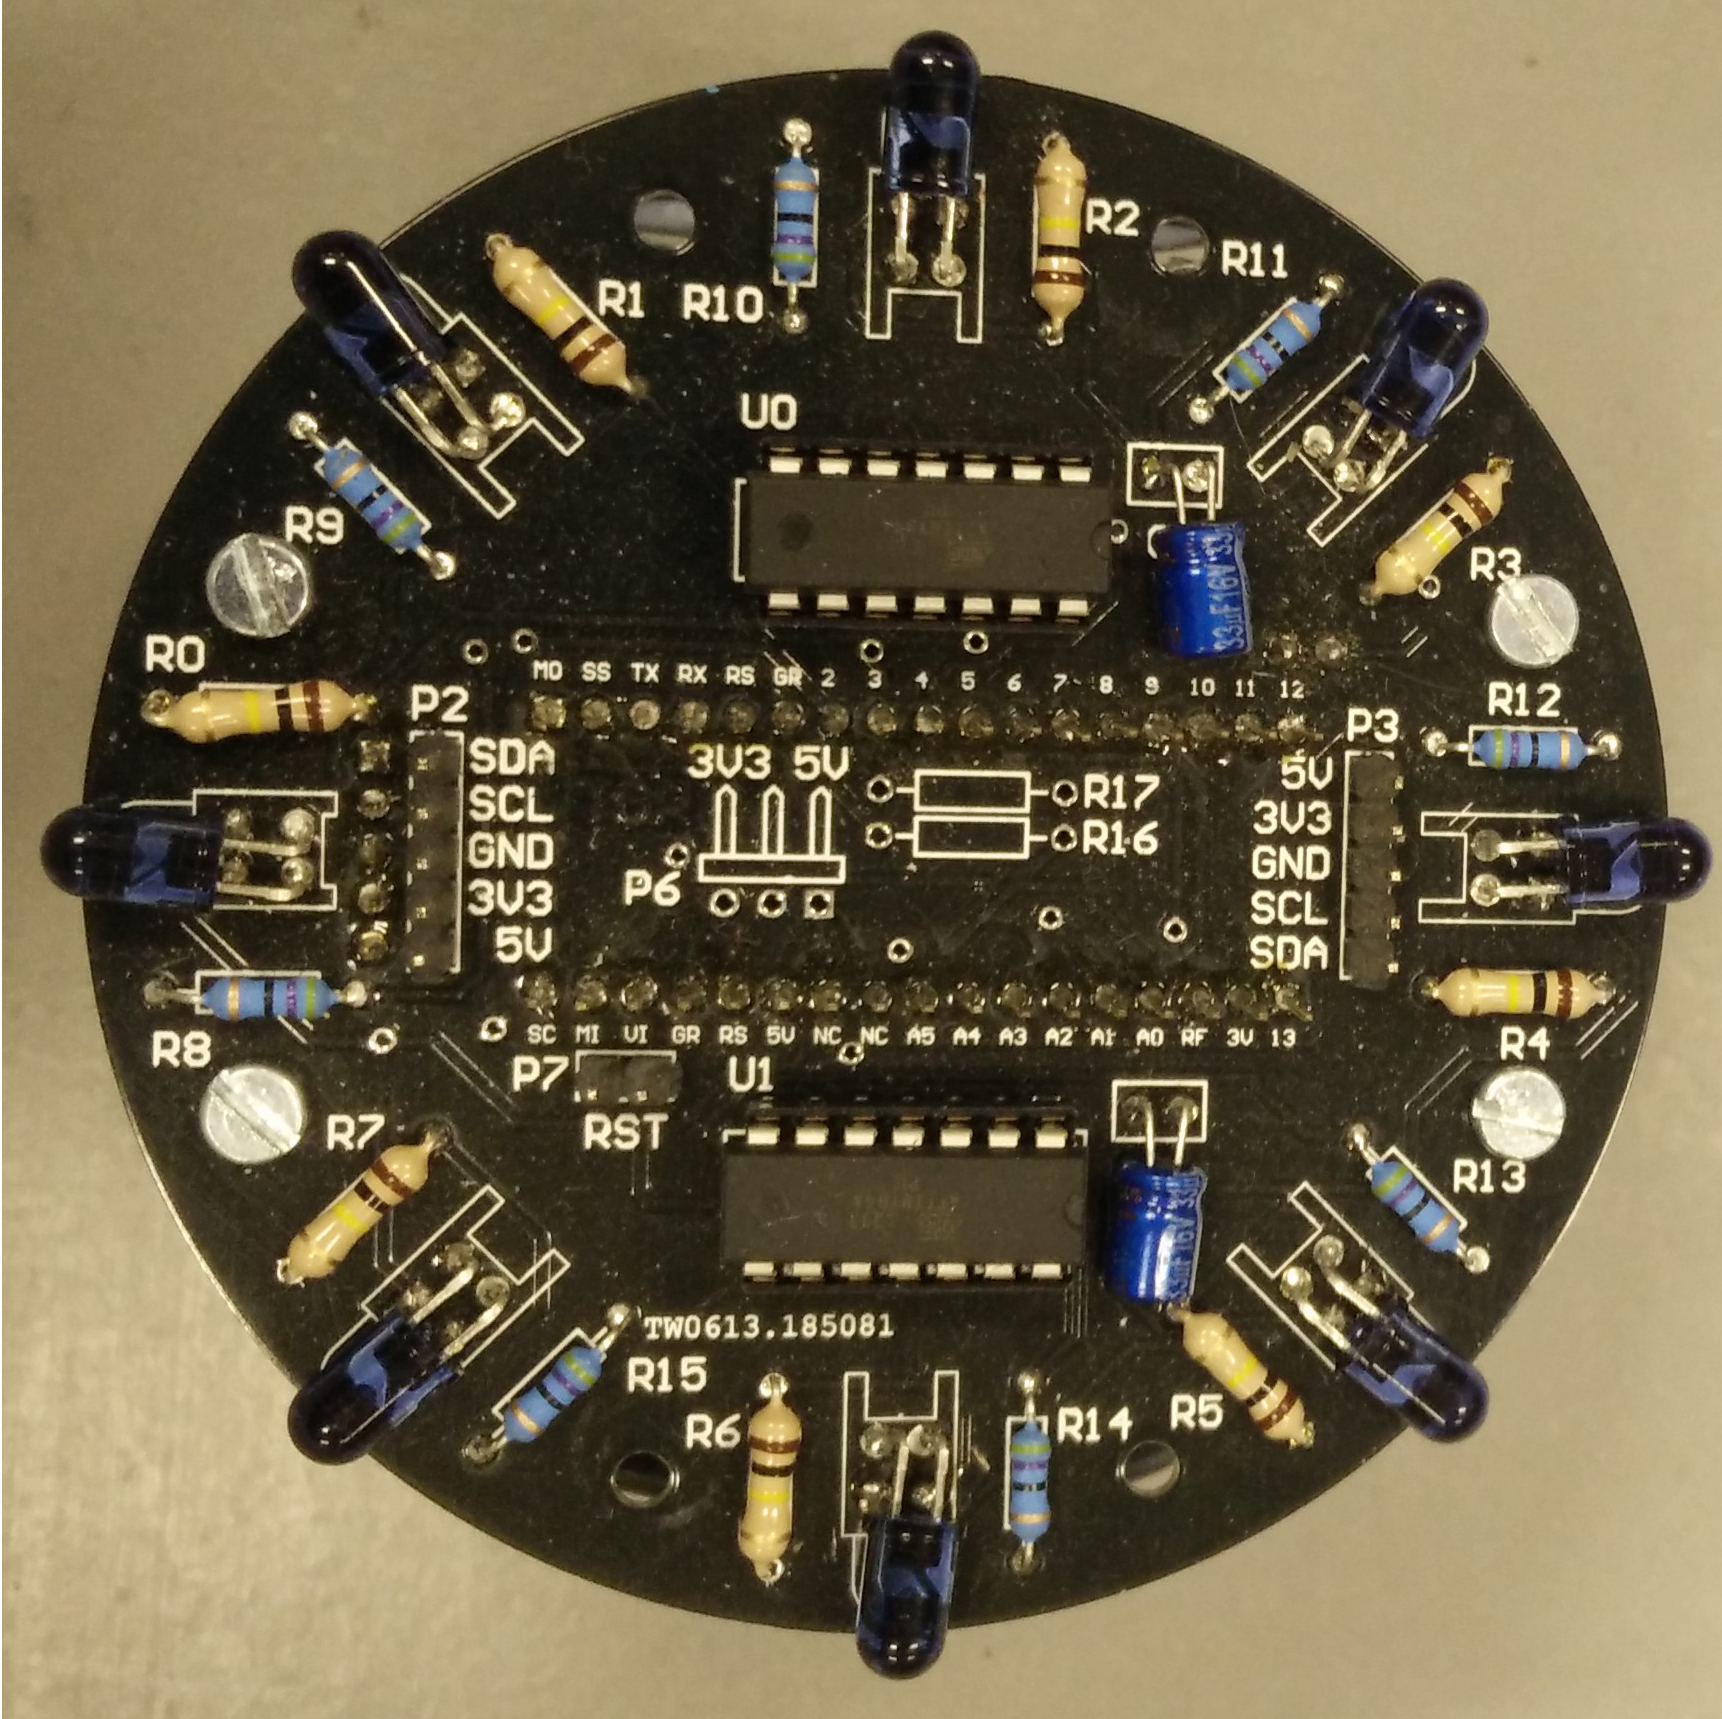
\includegraphics[width=0.8\linewidth]{images/chirpAbove.jpg}
\caption[ChIRP robot seen from above]{ChIRP robot seen from above, this one is equipped with 8 IR emitter and receivers}
\label{fig:chirpAbove}
\end{figure}
These can be used to measure distance by emitting the infrared light and measure how much of it is reflected back into the receiver. There are two ATtiny on top of the robot. ATtiny are a very simple microcontroller made by atmel. These ATtiny are programmed to handle the values found by the infrared receivers and converts them to a short (the datatype, 16 bit int) so the Arduino micro inside the ChIRP does not need to handle everything. This is due to the limited processor power of the Arduino micro which has a ATmega32u4 processor with 16 MHz clock speed and 32 KB flash memory. Arduino micro has 20 digital inpput/output (I/O) pins in which 7 of them are PWM, and 12 analog input pins. PWM stands for Pulse-width modulation \footnote{\href{http://arduino.cc/en/Tutorial/PWM}{http://arduino.cc/en/Tutorial/PWM}}, and those pins with PWM are able to emulate analog output by variating the high and low signal with various speed, also called modulation.
Inside the robot there's an ATtiny as well that helps the Arduino control the motors. These ATtinys that controls the motors and the 8 infrared receiver sensors needs to be programmed. The code is also available on the website. These ATtinys can be programmed using an Arduino Uno shield or by connecting the Uno to the ATtiny using a breadboard directly.
\begin{figure}[H]
	\centering
	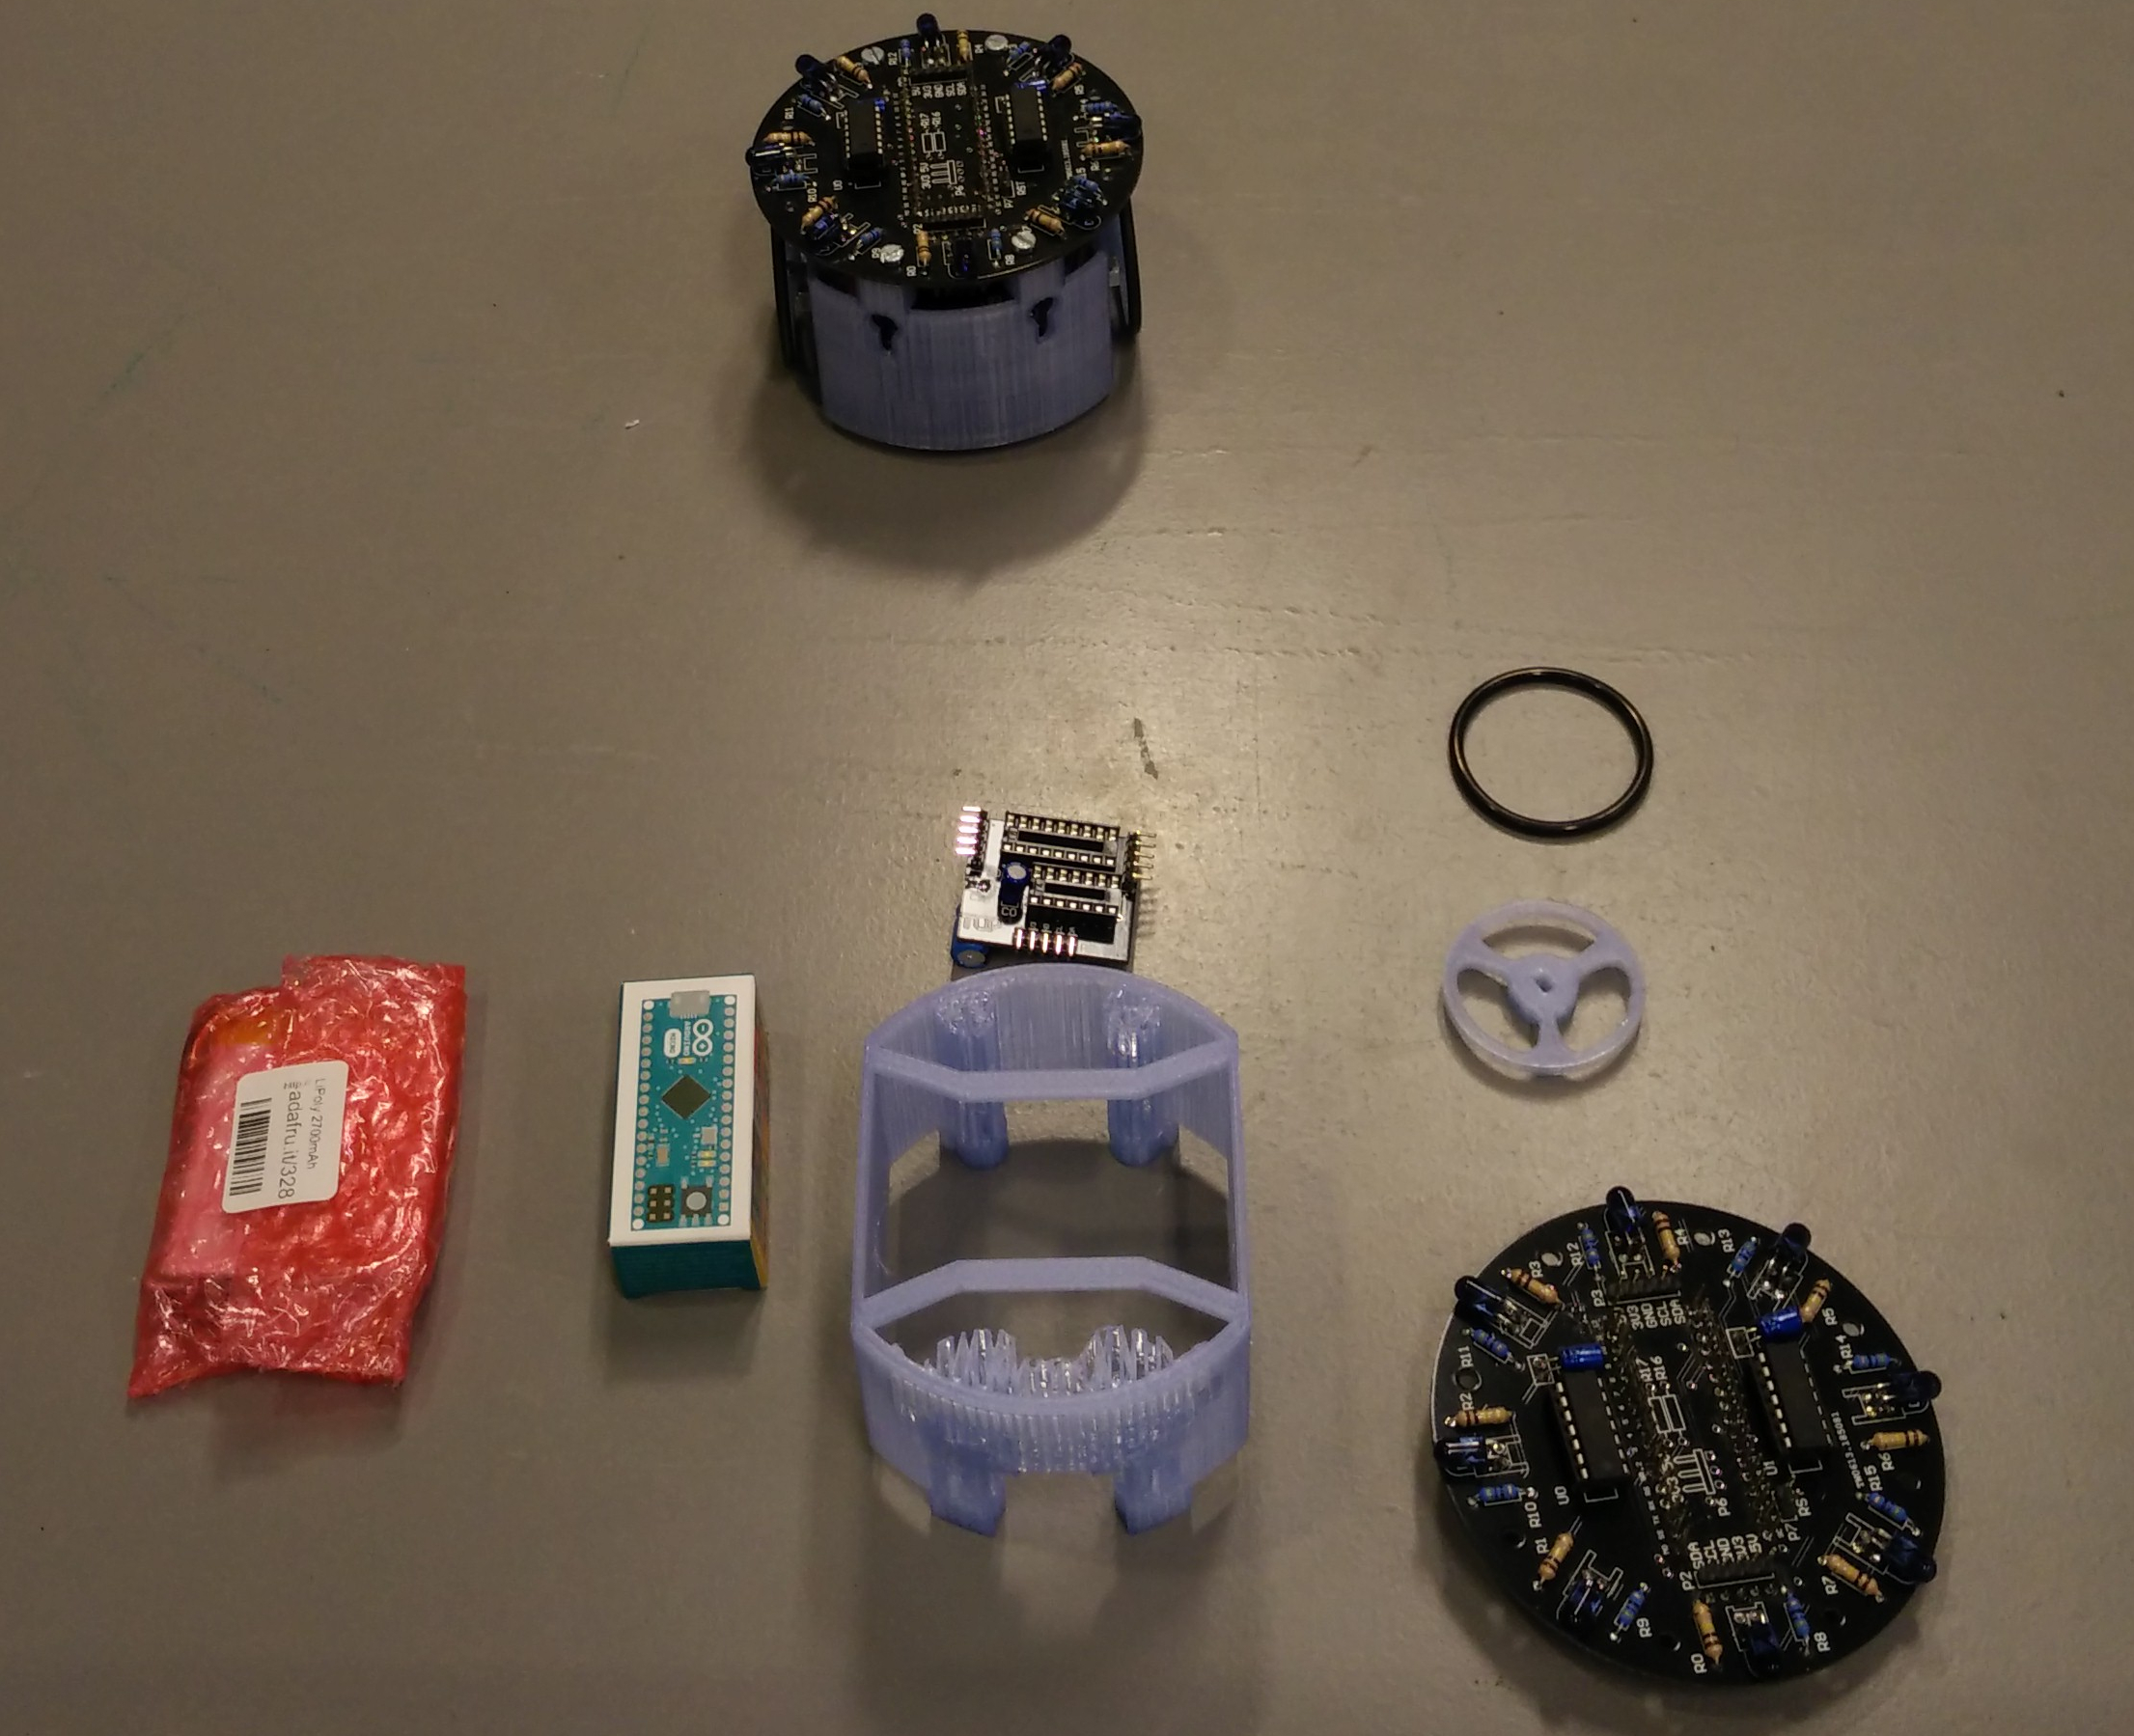
\includegraphics[width=0.8\linewidth]{images/chirpPieces}
	\caption[ChIRP pieces]{Some of the building blocks of the chirp robot}
\end{figure}


The ChIRPs are powered by a 3.7 volts 2500mAh battery which lasts for about 4.5 hours if they are running continuously, and it takes around 4 hours to recharge. The battery life can be increased if the robot is standing still. The batteries can be changed, but it can be quite difficult to do so due to the small gaps and the precision needed to connect the wires. The robots can be charged using a normal micro USB cable.




%4 preproject, what I did.
HSB
how platooning was implemented/3 sec rule

\section{Traffic Sim, pre-project}
For my master's pre-project I worked on a traffic simulator which controls the ChIRP robots.
The traffic simulator is a project for Statens Vegvesenet Teknologidagene in Trondheim where the ChIRP Robots were used to demonstrate the concept of platooning. 
The idea of platooning is to use an autonomous system (either global centralized system or each individual entity communicates with each other) to control the vehicles as one unit thus increasing the flow of traffic. These vehicles can be anything, but in this case we imagine them being cars or trucks found in traffic. When the red traffic light changes to green light, drivers usually drive one by one. The driver only drives forward when there's enough space in front of his or her car, in other words, the drivers are trying to follow the 3 second rule.
However with platooning and autonomous steering/driving the cars will drive instantly when the red light changes to green, and it will look like all the cars drive as one unit, or like a train if you will.
This leads to less air resistance and the cars will be able to cross an intersection much faster. This is considered dangerous if it had been normal humans driving, because driving with almost no gap in between the vehicles would not leave enough time to react and brake in time. With autonomous self driving vehicles it might be possible to platoon without being a risk because the cars can be considered as one unit, and when one car brakes or slow down all the cars behind it will start to brake/slowing down instantly without any reaction time added.

The system we used to demonstrate platooning for Vegvesenet Teknologidagen used a web camera to track all the robots in a sandbox. The sandbox is an empty box with four walls which the robots were able to move freely inside. Using a projector we drew an 8 shaped track on kraft paper which was later painted with black paint. Styrofoam was used to build a city-like environment around the track.
The combination of paint and kraft paper did not work very well due to bulges and the paint being too slippery for the robots, so they were not able to drive around efficiently. We therefore had to cut out the painted part, so the robots could drive on the sandbox floor.

All the robots were equipped with a bluetooth module and 2 circular post-it notes which was light green and pink.
The camera was able to detect these post-it notes using the OpenCV (Open source Computer Vision) and C++ boost library. The software for tracking the robots were already implemented and we only had to set it up on a xubuntu linux machine.
Using these pink and green post-it notes and a web camera, the computer could track the position and rotation of each robot. A parameter of how many robots had to be set beforehand, along with the parameters hue, saturation and brightness for the red (in our case pink) and green color. 
The position and rotation of each robot was then sent to the simulation written in Java via UDP packets as a string which the simulation decomposed using regular expression and converted to numbers which could be set for each robot. Due to the high update frequency of the camera, the simulator had to average each 5 position and rotation it got from the camera software. This was done to avoid jiggling due to noise. We had some problems with the camera software not working without a internet connection, the program would crash if the computer did not have an internet connection. The program needed it to send the packets over UDP, we had both camera software and Java simulation on the same machine, so the UDP packets were only sent to localhost so we did not really need a internet connection, but the software believed that it needed one. We fixed this problem by connecting a ethernet cable between the host machine and the computer nearby, that would trick the program thinking that it had a valid connection.
Another problem that was present was the ID of the robot, each robot would have an unique ID. When one of the robot went out of sight - that is the camera is being covered or the robot drove outside of its range, the camera software would assign new ID to all of the robots. For instance if we have 2 robots with the ID 0 and ID 1. If robot1 cannot be tracked by the camera then robot0 will get ID 2 and counting until robot1 reenters the frame. So at one point the robots might have the ID 7 and 8. The Java simulation uses these ID to keep track of the robots, and which COM port belongs to which ID. The simulator did still know approximately where each robot were supposed to be, so when a robot would disappear and reappear with a new ID, the simulator would simply find the nearest robot and reassign the ID to that robot.


The simulation then calculated where the robot needed to go, set the speed for each wheel and sent the commands to the robot using the bluetooth COM-port.

The Java simulation was first implemented by Magnus Hu using a game framework called Lightweight Java Game Library (LWJGL) to render everything on screen. We decided to change the framework from LWJGL to Slick2D. Slick2D is a 2D Java game library which uses tools and utilities wrapped around LWJGL, which means that it can do everything LWJGL can do, but also has higher abstraction. Slick2D lets us render shapes (circles, squares) without having to specify each point and line of the shape manually which we had to do in LWJGL. We could also easily check if the shapes intersected each other using the built in method "intersects" for the Shape class. In LWJGL, the robots were rendered as triangle by using 4 points, where 2 of the points would overlap. This was hard to build upon and it did not give an accurate model of how the robot looks in real life .
In Slick2D we rendered a circle shape for each robot with a square cone in front of it and a bit larger circle shape around the robot. The square cone was used as the vision of the robot, and the outer circular shape was used to detect when robots were too close to each other. If these out circles intersected the robot were forced to stop immediately because they are likely to crash into each other.\\


The track used in the simulation consisted of 24 points (a point as in a point in space) laid out in a 8-shaped layout, where the center intersection is made up of 2 points. For every point in the list, a line would be drawn between a point and its 2 neighbors in the list, this formed the 8-shaped figure which was our track.
A prototype image of a 8 shaped track that we got from Vegvesenet was used to find the 24 points. 
Our demo at Teknologidagene used 4 robots because we only had 4 bluetooth modules. The bluetooth modules had to be connected and added manually as a COM port before running the simulation or else it wouldn't know where to send the commands. When starting both the OpenCV camera tracking software and the simulation, the ID, coordinates of each robot and the rotation/alignment were tracked and sent via UDP packets. At this point in time, the simulation doesn't know which coordinate and rotation belongs to which bluetooth COM port. To map the COM port to a robot the simulator does the following for each robot:
\begin{itemize}
    \item checks the angle of all the robots
    \item sends a rotate command to the bluetooth COM port, which makes one robot rotate approximately 90 degrees.
    \item checks the angle of all the robots, finds out which one has rotated the most, saves this COM port to the robot which have rotated the most
    \item rotates the robot back to the original orientation
\end{itemize}
The reason for rotating the robot back to the original orientation is because we always laid the robot out in the map facing forward, which was easier to implement instead of implementing a lot of code to ensure that the robot would face forward if it started out in the wrong direction.
Each robot will now have a COM port given that the COM port didn't time out on initiation, in which we had to restart the whole simulation program to reconnect to the COM port.
The simulation then calculates the robot's nearest point on the track, and sets the target point of the robot to be point after the nearest one, this is in case the nearest point is behind the robot. After the simulation found out where the robot should move to, it calculates which way the robot needed to rotate and which speed it should have. The speed and the amount of needed rotation ($\Delta angle$) is then converted to <"two motors"> which is sent as a byte array of 4 elements to the robot's bluetooth module. An example of the byte array could be "l40r50" which means that the right motor would drive a little bit faster than the left one thus turning the robot to the left.
If we used a capital 'L' or 'R' in the byte array instead, the wheel would turn backwards, however we don't use that in the simulation at all except for turning the robot in the beginning when it tries to assign the COM port to the correct robot.

The simulator creates a box in front of each robot that will be used to find out whether the robot has a robot in front of it or not. If there's a robot in front (that is inside the front box) then the simulator will check if platooning is on or not. If platooning mode is on, the robot will try to keep the same speed as the robot in front of it. At least it's not allowed to have higher speed than the robot in front of it, or else it will crash into it. If platooning mode is off, then the robot will try to keep a 3 second distance from the robot in front, that is the robot will try to keep the robot in front of it outside the detection box. The robot is considered as reaching a target if the robot's center is 20 pixels away from the target, and the next point will be assigned as the new target for the robot.
The simulator have two modes for the robot, one where platooning is activated and one mode where the robots behave like normal cars. The normal car mode is emulating how drivers would drive normally. In front of each robot in the simulation there would be rendered a square cone-shaped shape which would be larger when the robot had high speed and smaller if the robot had slower speed. The shape would be almost non existing if the robot were to stand completely still. This shape would tell the robot that there is another robot in front of it, and the current robot would try to adjust it speed so the robot in front is outside of this "detector" shape. This shape is supposed to be a three second rule, and would let the robot brake without having to brake heavily.
In platooning mode on the other hand, the robots will extend their shape a lot further than it did in normal drive mode. This shape will now be used to ask the robots inside of it what speed they have, and if they're braking or not.
If the robot in front have a max speed $x$ then the robot behind can only drive as fast as $x$, a higher speed would make the robot crash or bump into each other.
The robot in the back will always ask the robot in front if it is braking or not, if the robot in front says that it is currently braking, then the robot behind would also brake immediately.
In our implementation we had to cheat the platooning algorithm a bit, due to the delays in the bluetooth signals and how fast the robots are able to react. If we sent a new command too rapidly, the robot would not move because a new command would overwrite the old command before the motors were able to issue the old command. So we had to insert a delay between sending each command to the robots, we were only allowed to send a command 5 times each second. This was enough to make the platooned robots fall a little bit behind the robot in front of it, so it did not seem like they platooned at all. The fix we implemented was to have the cars behind try to catch up to the robot in front of it if the current mode was platooning mode. This fix made the robots look more like they actually were platooning.\\

Some other problems we had under the demonstration was some of the styrofoam buildings used around the tracks were too tall, and covered the robots when they rounded the turn. When we cut down the tallest building, it was still casting shadows on to the track. The shadow made the robot's post it note have a different shade of green/pink, and the camera lost track of it. We had to cut the building even more so the shadow didn't reach the track.


In the middle of the map, at the intersection there is a red light at the top, north side or at the right, east side of the intersection. This red light will be alternating between these two positions depending on what the user chooses. 

Most of the codes written for this platooning demo was already implemented or had already been started on, the code for the robot tracking written in C++ with the openCV and boost library. The libraries for the ChIRP robot already existed, Christian Skjetne implemented the code using Arduino language on the robot which used the bluetooth module. 
I did not get to code so much on the robots itself, but next semester I will be a student assistant in the new course for the first grader in computer science named programming lab where they are supposed to program on the Arduino. So this year I have been attending two courses that focused on learning input sensors and getting to know the Arduino. One of the main thing in that course is the bluetooth low energy module, which is pretty similar to the bluetooth used on the ChIRPs. 

%5 master project
\section{Master project}
For my master project and thesis I will try to implement the Boids behavior on the ChIRP robots. The robots have 8 IR-LEDs and 8 IR receivers which I will use to avoid obstacles and the walls. The ChIRP robots can easily detect colored obstacles, but have some problems with black objects because they do not reflect light very well. The same goes for other robots, they do not reflect infrared light very well, due to the structure of the robots. The robot is pretty hollow at the top, where the infrared LED lights are mounted. This might impose a problem with object avoidance or the Boids' separation behavior. The quick fix for this is to physically alter the robot by adding a paper strip around robot, near the IR-LEDs which will hopefully reflect the infrared light.
The robots' PCB also have holes in it that we can use to mount various other things on top of it. These holes can be used to mount some sort of reflectors that will reflect the infrared light if the paper method does not work.
\begin{figure}[H]
\centering
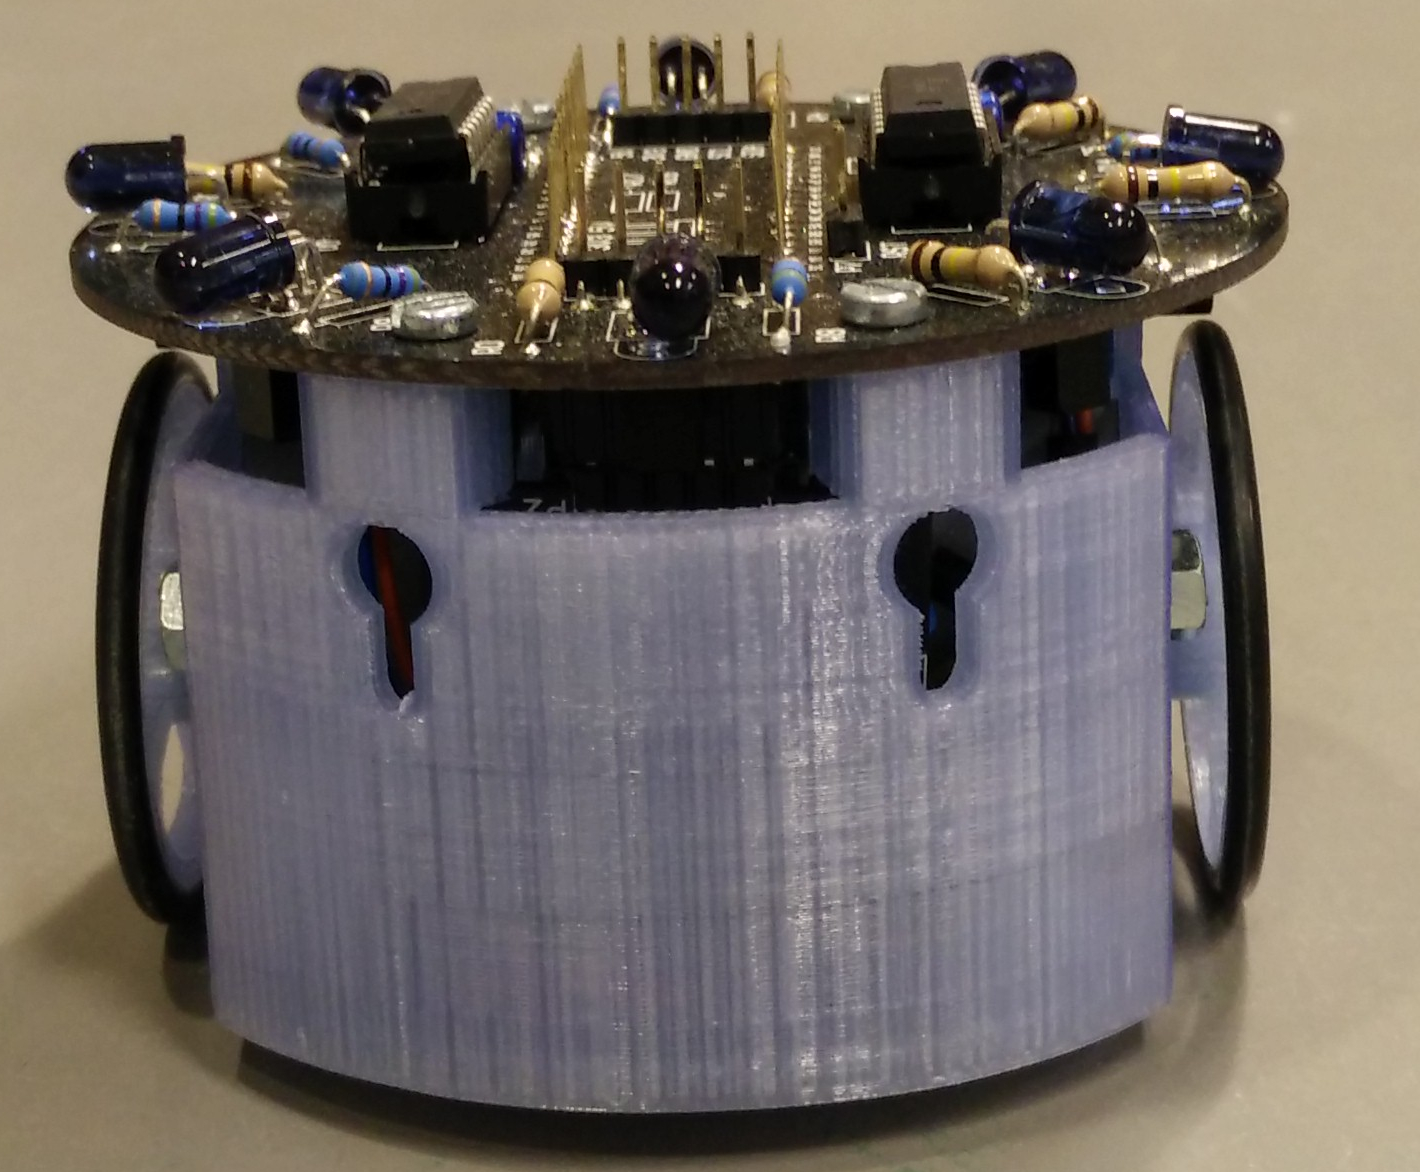
\includegraphics[width=0.8\linewidth]{images/chirpFront.jpg}
\caption[Front of ChIRP robot]{The front of the ChIRP robot, the blue IR LED on top of the robot might not reflect as good of other robots due to the structure of it}
\label{fig:chirpsFront}
\end{figure}
For now we only have 4 functional bluetooth modules that the robots can use. We have all in all 6 bluetooth modules, but we lack adapters. It is not possible to connect the bluetooth modules to the robot without these adapters. New adapters can be printed in Omega-verksted or bought from companies that prints out PCB.

Only using the IR distance sensors is not enough to find all the information needed to implement Boid behavior on the robot, namely the position of each robot and their rotation.
Each robot will therefore communicate with a computer using their bluetooth module.
This centralized computer will have an overview of the sandbox using the web camera and the tracking software found in the SVN repository and will be able to provide the robots with the information they need.

Swarming robots are not supposed to communicate with an overall centralized system, but due to the technical limitation and sensors each robot is equipped with, the alternative to communicating with a centralized system is to equip more advanced sensors on the robot, which might not be plausible.

After simple Boid behavior is implemented, I will try to implement different type of steering behaviors mentioned in the steering paper. If there is enough time, I would like to assemble some of the ChIRP robots so I can get to know the inner workings of the robots. The ChIRP robots can easily be expanded with more sensors, it would be fun to implement fleeing and pursuit behavior based on for instance the light sensors or something similar, that way we do not need to use a centralized system to tell the robots which position they need to go to or flee from.

It is also possible to create complex mazes using the projector and the camera to detect these drawings, or using the robots' light sensors to differentiate between black spots and white light on the sandbox. This can be used for path following for instance.

These robots can only move forward, backward and/or rotate. They cannot move sideways. I do not know if that will impose a problem, but real birds and particles in simulation are allowed to move sideways, for the separation behavior as shown in figure \ref{fig:boid_sep} it seems like the Boid is moving sideway. The robot might have to turn around, move in that direction and the turn back.

Before testing anything on the robots, I will need to create a simulation where I will be able to test and debug. A simulation would able to provide information that the real robots are not capable of providing, and thus it will be easier to see if the individuals are behaving like they are supposed to do. A lot of the code from the traffic simulation can be reused, but I would rewrite the Robot class, this is because the old Robot class were written with speed and rotation, instead of 2 wheel drive.

The Arduino have limited memory, only 32 KB are present on the micro board. I do not think I will exceed this limitation, but if my implementation exceed this memory cap, then I need to rewrite the code to use smaller data types. For instance a normal \textbf{int} uses 32 bits, but one might not need all of the 32 bits. It would be better to use a \textbf{byte} data type instead, which only uses 8 bits.



%references
\pagenumbering{Roman}
\nocite{*}
\bibliographystyle{plain}
\bibliography{bibl}
\newpage
%appendix
\section{Appendix}
\label{sec:app}
\appendix

\pagenumbering{Alph}
	\chapter{Camera tracking configuration file}
\label{app:opencvcfg}
chirpObserverConfig.cfg
\begin{lstlisting}
# [comPort]
# the id of the comm port to use. 
# 0 corresponds to /dev/ttyS0 
# 1 corresponds to /dev/ttyS1
# 2 corresponds to /dev/ttyS2
# 3 corresponds to /dev/ttyS3
# 4 corresponds to /dev/ttyS4
# 5 corresponds to /dev/ttyS5
# 6 corresponds to /dev/ttyS6
# 7 corresponds to /dev/ttyS7
# 8 corresponds to /dev/ttyS8
# 9 corresponds to /dev/ttyS9
# 10 corresponds to /dev/ttyS10
# 11 corresponds to /dev/ttyS11
# 12 corresponds to /dev/ttyS12
# 13 corresponds to /dev/ttyS13
# 14 corresponds to /dev/ttyS14
# 15 corresponds to /dev/ttyS15
# 16 corresponds to /dev/ttyUSB0
# 17 corresponds to /dev/ttyUSB1
# 18 corresponds to /dev/ttyUSB2
# 19 corresponds to /dev/ttyUSB3
# 20 corresponds to /dev/ttyUSB4
# 21 corresponds to /dev/ttyUSB5
# 22 corresponds to /dev/ttyAMA0
# 23 corresponds to /dev/ttyAMA1
# 24 corresponds to /dev/ttyACM0
# 25 corresponds to /dev/ttyACM1
# 26 corresponds to /dev/rfcomm0
# 27 corresponds to /dev/rfcomm1
# 28 corresponds to /dev/ircomm0
# 29 corresponds to /dev/ircomm1
# id = 27

[camera]
# the id of the camera device to use, numbered from 0 and upwards
# deviceId = 1
deviceId = 0
# the width and height of the captured image, denoted in pixels
width = 720	
height = 500
# the maximum number of objects to track. 
#All objects are ignored if the number of objects
# discovered exceeds this number
maxNumObjects = 1000
#the minimum object area to recognize (in pixels). 
#Any object smaller than this is ignored.
minObjectArea = 10
# upper limit of the size of leds compared to 
# min(frame width, frame height)
ledSize = 0.01

# settings governing the colors in the captured frame
# the settings are potentially specific to each camera
# linux application "guvcview" provides details
# the settings appear to be sticky, so an application like 
#"guvcview" may be necessary to revert to default state
#
# if the value is less than 0, the application won't change
# the camera's setting for that property
# the brigtness of the image
brightness = 0.1
# the contrast of the image (0 - 10 with default of 5)
contrast = 5
# the saturation of the image (0 - 200 with default of 83)
saturation = 30

# each color is defined by six boundries,
#and is only recognized if the HSV value is within the bounds
[red]
hmin = 120
hmax = 220
smin = 100
smax = 256
vmin = 130
vmax = 256

#hmin = 0
#hmax = 45
#smin= 90
#smax = 256
#vmin = 170
#vmax = 256

[blue]
hmin = 100
hmax = 120
smin = 250
smax = 256
vmin = 250
vmax = 256

[green]
hmin = 31
hmax = 90
smin = 100
smax = 256
vmin = 135
vmax = 256

#hmin = 21
#hmax = 86
#smin= 50
#smax = 256
#vmin = 205
#vmax = 256

# the size of the virtual feed depicting the 
#scene as interpreted by the tracker
[virtualFeed]
width = 500
height = 500
 
# settings for the UDP network sending 
#information about tracked robots
[network]
enabled = true 
address = localhost
port = 52346

[general]
# whether to calibrate colors, this allows one to 
#find values for the color definitions
calibrationEnabled = false
# the time the system waits after a frame 
#has been processed before it fetches a new one
# if this number is set too low, 
#the camera won't be able to finish capturing a frame
frameDelay = 10

[tracking]
# number of robots to track
numRobots = 4
# robots are removed if this number of steps pass 
#without a pinpointing of the robot's position
evictionLimit = 6
# the maximum speed (distance / frame) of robots in any 
#direction compared to the width and height of the bounding box
 robotSpeed = 0.01
# robotSpeed = 0.065
# the maximum rotational speed (radians / frame) of
# the robot compared to a full circle
robotRotationalSpeed = 0.05
# the diameter of the robots compared to the bounding box
robotDiameter = 0.06
#0.059
# the number of recent values to use when smoothing
# the position and rotation of the robot
historyLength = 3

[controls]
# key to reload the configuration at run time. 
#Not all changes will take effect
loadConfig = l
\end{lstlisting}
	\chapter{Sorting algorithms}
\label{app:sorting} This section will explain some of the sorting algorithms that are used in some of the papers mentioned in chapter \ref{sec:background}. 
\section{Odd even sort}
Odd even sort is a sorting algorithm which resembles bubble sort. The algorithm takes a list of elements, then compares all the odd placed element with the element next to it. That is; compare list[i] with list[i+1] where $i$ is an odd number. Then the algorithm does the same for all $i$ even number. This is done repeatedly until we get a sorted list.

\section{Bitonic sort}
Bitonic sort is a highly parallel sorting algorithm, the idea is to have the elements in the list in a bitonic sequence. A bitonic sequence is a sequence where the list is increasing, then decreasing and then eventually increasing again. However the last increasing part are not allowed to increase past the first element in the list.
\begin{figure}[H]
    \centering
    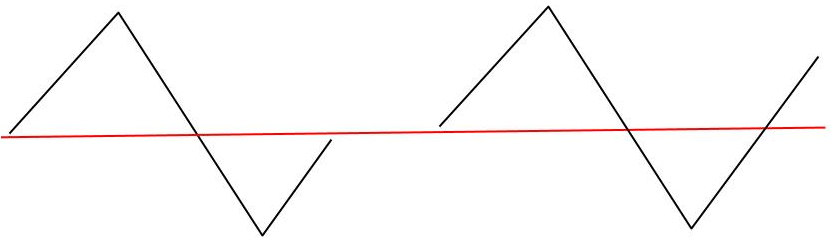
\includegraphics[width=0.8\linewidth]{images/bitonicseq}
    \caption[Sequence of elements]{Left figure is a bitonic sequence, right figure is not a bitonic sequence because the last increasing part is higher than the start}\label{fig:bitonicseq}
\end{figure}
After the algorithm have obtained a bitonic sequence, it will start to compare the elements with certain distance from each other and swap these elements if they are in the wrong order.
\begin{figure}[H]
    \centering
    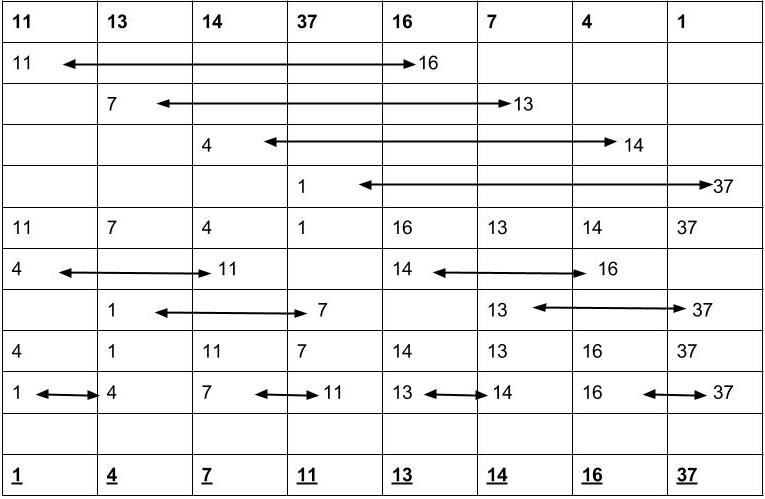
\includegraphics[width=0.8\linewidth]{images/bitonicexample}
    \caption{Example of a bitonic sort run}\label{fig:bitonicex}
\end{figure}
In the example we have the numbers 11,13,14,37,16,7,4,1. Which is initially in a bitonic sequence because the first half is increasing and the last half is decreasing. The algorithm now compares the first and the fifth element, as indicated by the arrows. All of these comparisons can be done in parallel. The algorithm compares the elements at different position, in the example it start with a comparison of elements that are distance 4 away from each other, that is element at position 1 and 5, 2 and 6 and so on. Then elements with distance 2 is compared, and then elements with distance 1 are compared.
The runtime of the bitonic sort algorithm is $O(nlog(n)^2)$ but the idea is to run it on $n$ Cuda threads, reducing the runtime to $O(log(n)^2)$ for each thread.


\end{document}
